\documentclass[compress]{beamer}
\usecolortheme{default}

\usepackage{lmodern, epstopdf, multirow, array, setspace, bbm, tcolorbox, pbox, bm, mathtools, tikz}
\usepackage[T1]{fontenc}

\setbeamertemplate{frametitle}[default][center]
\setbeamertemplate{footline}{\hfill \insertframenumber/\inserttotalframenumber\hspace*{5pt}\vspace{5pt}}
\setbeamertemplate{navigation symbols}{}

\newlength{\wideitemsep}
\setlength{\wideitemsep}{\itemsep}
\addtolength{\wideitemsep}{4pt}
\let\olditem\item
\renewcommand{\item}{\setlength{\itemsep}{\wideitemsep}\olditem}
\setlength{\leftmargini}{12pt}
\setlength{\leftmarginii}{14pt}
\setbeamertemplate{itemize/enumerate subbody begin}{\vspace{6pt}}
\setbeamertemplate{itemize item}[circle]
\setbeamertemplate{enumerate item}[circle]
\setbeamertemplate{enumerate subitem}[default]

\setbeamercolor{alerted text}{fg=blue}
\setbeamersize{text margin left=1.5em,text margin right=1.5em}

\tcbset{
    colback=white,
    colframe=black,
    coltext=black,
    coltitle=blue,
    colbacktitle=white,
    boxrule=1pt,
    titlerule=0pt,
    toptitle=4pt,
    top=2pt
}

\newenvironment{changemargin}[2]{% 
  \begin{list}{}{% 
    \setlength{\topsep}{0pt}% 
    \setlength{\leftmargin}{#1}% 
    \setlength{\rightmargin}{#2}% 
    \setlength{\listparindent}{\parindent}% 
    \setlength{\itemindent}{\parindent}% 
    \setlength{\parsep}{\parskip}% 
  }% 
  \item[]}{\end{list}}
  
\newenvironment{defn}{%
  \begin{tcolorbox}[title={Definition}]%
  }{\end{tcolorbox}}
  
\newenvironment{prop}[1]{%
  \begin{tcolorbox}[title={Proposition #1}]%
  }{\end{tcolorbox}}
  
\newcommand{\cit}[1]{{\footnotesize \textcolor[rgb]{0.5,0,0}{#1}}}

% Font size for code listings (verbatim blocks); reset with \normalsize
\newcommand{\codesize}{\fontsize{7}{8.5}\selectfont}

\newcommand{\slidesetup}[1]{%
  \title{#1}%
  \subtitle{\texorpdfstring{\vspace{0.3\baselineskip}}{} {\small This version: \today}}%
  \author[Mikkel Plagborg-Moller]{ECMA 31150, Spring 2026 \texorpdfstring{\\[0.5ex]}{} University of Chicago \texorpdfstring{\\[0.5ex]}{} Department of Economics \texorpdfstring{\\[4ex]}{} Mikkel Plagborg-Moller}%
  \date{}%
}

% \circleoverlay[options]{text}
% Draws a red circle with a text box nearby on a tikz overlay.
% Options (with defaults):
%   cx=0cm, cy=0cm      - circle center (shift from page center)
%   r=1cm               - circle radius
%   tx=0cm, ty=0cm      - text box offset from circle center
%   text anchor=east    - anchor of text node (east = text left, west = text right)
%   font=\normalsize    - font size for text
\pgfkeys{
  /circleoverlay/.cd,
  cx/.store in=\cocx, cx=0cm,
  cy/.store in=\cocy, cy=0cm,
  r/.store in=\cor, r=1cm,
  tx/.store in=\cotx, tx=0cm,
  ty/.store in=\coty, ty=0cm,
  text anchor/.store in=\cotextanchor, text anchor=east,
  font/.store in=\cofont, font=\normalsize,
}
\newcommand{\circleoverlay}[2][]{%
  \pgfkeys{/circleoverlay/.cd, cx=0cm, cy=0cm, r=1cm, tx=0cm, ty=0cm, text anchor=east, font=\normalsize, #1}%
  \pgfmathsetlengthmacro{\circlediameter}{2*\cor}%
  \node[draw=red, line width=2pt, circle, minimum size=\circlediameter, inner sep=0pt]
    (tmpcirc) at ([xshift=\cocx,yshift=\cocy]current page.center) {};%
  \node[anchor=\cotextanchor, fill=white, draw=red, text=red, inner sep=4pt, align=left, font=\cofont]
    at ([xshift=\cotx,yshift=\coty]tmpcirc.center) {#2};%
}

\DeclareMathOperator*{\argmax}{argmax}
\DeclareMathOperator*{\argmin}{argmin}
\DeclareMathOperator{\diag}{diag}
\DeclareMathOperator{\var}{Var}
\DeclareMathOperator{\cov}{Cov}
\DeclareMathOperator{\corr}{Corr}
\DeclareMathOperator{\lrv}{LRV}


\slidesetup{Dynamic causal effects II}

\begin{document}
\frame{
\maketitle
}

\frame{
\frametitle{Plan for this slide deck}
\begin{enumerate}
\item Quantifying the importance of shocks
\item Examples of shock measurement in the applied literature
\item Dealing with measurement error in the shock
\item Small-sample bias of LP
\item Panel LP
\end{enumerate}
}

\frame{
\frametitle{How important are climate shocks?}
\begin{itemize}
\item Consider again the Bilal \& K\"{a}nzig (2026) application from the previous slide deck.
\item We have estimated the dynamic causal effects (i.e., IRF) of world GDP wrt.\ climate shocks.
\item But world GDP depends on many other kinds of shocks, too.
\item We would like to quantify how \emph{important} our (residualized) shock $\tilde{x}_t$ is for the outcome $y_t$, relative to everything else that drives $y_t$.
\end{itemize}
}

\frame{
\frametitle{Forecast error variance decomposition}
\begin{itemize}
\item \textbf{Forecast error variance decomposition} (FEVD): how much would the $h$-step-ahead MSFE $E[(y_{t+h}-y_{t+h|t})^2]$ decrease if we hypothetically knew the intervening shocks $\tilde{x}_t,\dots,\tilde{x}_{t+h}$ in advance?
\item Estimation procedure (separately for each horizon $h$):
\begin{enumerate}
\item Regress $y_{t+h}$ on all control variables $\bm{r}_t,\bm{w}_{t-1},\dots,\bm{w}_{t-p}$. Compute the (forecast) residual $e_{t+h|t}$.
\item $\mathit{FEVD}_h \equiv R^2$ from regression of $e_{t+h|t}$ on $\tilde{x}_t,\tilde{x}_{t+1},\dots,\tilde{x}_{t+h}$. 
\end{enumerate}
\item Note: this definition depends on the set of controls. We're asking how well current+future $\tilde{x}_t$ explain the forecast error from the regression with baseline controls.
\end{itemize}
}

\begin{frame}[fragile]
\scriptsize
\begin{verbatim}
# Leads of residualized shock
for l in range(max_horizon + 1):
    df[f'temp_anom_resid_lead{l}'] = df['temp_anom_resid'].shift(-l)

# Estimate FEVD
fevd = np.empty(max_horizon + 1)
for h in range(max_horizon + 1):
    y = df['l_gdp'].shift(-h)
    reg1 = sm.OLS(y, sm.add_constant(df[control_cols]), missing='drop').fit()
    cols = [f'temp_anom_resid_lead{l}' for l in range(h + 1)]
    reg2 = sm.OLS(reg1.resid,
                  sm.add_constant(df.loc[reg1.resid.index, cols]),
                  missing='drop').fit()
    fevd[h] = reg2.rsquared
\end{verbatim}
\end{frame}

\begin{frame}[fragile]
\begin{verbatim}
        FEVD
h           
0   0.017150
1   0.023892
2   0.061400
3   0.113741
4   0.160317
5   0.226175
6   0.302844
7   0.324311
8   0.273270
9   0.267634
10  0.266006
\end{verbatim}
\uncover<2>{%
\begin{tikzpicture}[overlay, remember picture]
  \circleoverlay[cx=-4.2cm, cy=-0.9cm, r=1cm,
                 tx=1.5cm, ty=0cm, text anchor=west]{Climate shocks explain 32\% of \\ GDP forecast variance 7 years out!}
\end{tikzpicture}%
}
\end{frame}

\frame{
\frametitle{Examples of shock measurement in the applied literature}
\begin{enumerate}
\item Romer \& Romer (1989, 2004) combine information from the meeting transcripts of the Federal Open Market Committee (FOMC) with data on the Fed's expectations of future economic conditions to isolate the ``exogenous'' components of changes in the federal funds rate.
\item Gertler \& Karadi (2015) measure a monetary shock as the high-frequency movement in futures prices in a 30-minute time window around FOMC announcements.
\item Miranda-Agrippino, Hac{\i}o\u{g}lu-Hoke \& Bluwstein (2025) measure productivity news shocks using patent application data.
\end{enumerate}
\bigskip
\begin{itemize}
\item All these are likely to contain some \textbf{measurement error}: errors in interpreting the Fed meetings, financial micro-structure noise, patents as imperfect measures of ideas, etc.
\end{itemize}
}

\frame{
\frametitle{Proxies}
\begin{itemize}
\item Suppose we have constructed a direct measure $z_t$ of an underlying shock $\varepsilon_{1t}$, but it's contaminated with measurement error $\xi_t$:
\[z_t = \gamma \varepsilon_{1t} + \xi_t.\]
We call $z_t$ a \textbf{proxy} or \textbf{external instrument} for $\varepsilon_{1t}$.
\item Proxy assumptions:
\begin{enumerate}
\item \textbf{Relevance:} $\gamma \neq 0$. The proxy is informative about $\varepsilon_{1t}$.
\item \textbf{Dynamic exogeneity:} $\cov(\xi_t,\varepsilon_{js})=0$ for all $j,s$. The noise $\xi_t$ is unrelated to any systematic economic shocks.
\end{enumerate}
\end{itemize}
}

\frame{
\frametitle{Proxies: attenuation bias}
\[z_t = \gamma \varepsilon_{1t} + \xi_t\]
\vspace{-\baselineskip}
\begin{itemize}
\item Recall the representation we derived in the previous slide deck:
\[y_{t+h} = \mu + \Theta_{h1}\varepsilon_{1t} + v_{h,t+h}.\]
\item A simple LP of $y_{t+h}$ on $z_t$ suffers from \textbf{attenuation bias}:
\[\hat{\beta}_h \equiv \frac{\widehat{\cov}(y_{t+h},z_t)}{\widehat{\var}(z_t)} \overset{p}{\to} \frac{\cov(y_{t+h},z_t)}{\var(z_t)} = \Theta_{h1} \underbrace{\frac{\gamma \var(\varepsilon_{1t})}{\gamma^2 \var(\varepsilon_{1t}) + \var(\xi_t)}}_\text{bias factor},\]
since $\cov(v_{h,t+h},\xi_t)=\cov(\varepsilon_{1t},\xi_t)=0$ for classical meas.\ error.
\item Intuitively, a 1-unit increase in $z_t$ does not correspond to a 1-unit increase in the unobserved shock $\varepsilon_{1t}$ -- there is also noise.
\item Problem: the bias factor is not estimable.
\end{itemize}
}

\frame{
\frametitle{Proxies: attenuation bias (cont.)}
\begin{itemize}
\item Solution to the bias problem: normalize the scale of the shock using another observed variable $\bar{y}_t$ (the \textbf{normalization} variable).
\item If $\bar{y}_t$ also satisfies an SVMA model, then
\[\bar{y}_t = \bar{\mu} + \bar{\Theta}_{01}\varepsilon_{1t} + \bar{v}_{0,t},\]
where $\bar{\Theta}_{01}$ is the impact impulse response of $\lbrace \bar{y}_t \rbrace$ wrt.\ $\lbrace \varepsilon_{1t} \rbrace$.
\item Let $\hat{\beta}_{h,z\to y}$ be the coefficient in an LP of $y_{t+h}$ on $z_t$ (previous slide). 
\item Let $\hat{\beta}_{0,z\to \bar{y}}$ be the coefficient in an LP of $\bar{y}_t$ on $z_t$.
\item Then, by the calculation on the previous slide,
\[\frac{\hat{\beta}_{h,z\to y}}{\hat{\beta}_{0,z\to \bar{y}}} \overset{p}{\to} \frac{\Theta_{h1} \times (\text{bias factor})}{\bar{\Theta}_{01} \times (\text{bias factor})} = \frac{\Theta_{h1}}{\bar{\Theta}_{01}},\]
since the bias factor depends only on the proxy, not the outcome.
\end{itemize}
}

\frame{
\frametitle{Proxies: unit effect normalization}
\[\frac{\hat{\beta}_{h,z\to y}}{\hat{\beta}_{0,z\to \bar{y}}} \overset{p}{\to} \frac{\Theta_{h1}}{\bar{\Theta}_{01}}\]
\begin{itemize}
\item Conclusion: the ratio $\hat{\beta}_{h,z\to y}/\hat{\beta}_{0,z\to \bar{y}}$ of two LP coefficients estimates the \emph{relative} impulse response $\Theta_{h1}/\bar{\Theta}_{01}$.
\item $1/\bar{\Theta}_{01}$ = how big of a shock $\varepsilon_{1t}$ you need in order to raise $\bar{y}_t$ by 1 unit on impact.
\item $\Theta_{h1}/\bar{\Theta}_{01}$ = causal effect on $y_{t+h}$ of a shock $\varepsilon_{1t}$ of a magnitude that raises $\bar{y}_t$ by 1 unit (on impact).
\begin{itemize}
\item This normalization of the magnitude of the shock is called the \textbf{unit effect normalization}.
\end{itemize}
\item Unit-effect-normalized impulse responses are convenient to interpret.
\end{itemize}
}

\frame{
\frametitle{LP-IV}
\[\frac{\hat{\beta}_{h,z\to y}}{\hat{\beta}_{0,z\to \bar{y}}} \overset{p}{\to} \frac{\Theta_{h1}}{\bar{\Theta}_{01}}\]
\begin{itemize}
\item We have seen that we can estimate unit-effect-normalized impulse responses as the ratio of two LPs: $z \to y$ and $z \to \bar{y}$.
\item Rather than explicitly running two LPs, notice that
\[\frac{\hat{\beta}_{h,z\to y}}{\hat{\beta}_{0,z\to \bar{y}}} = \frac{\widehat{\cov}(y_{t+h},z_t)/\widehat{\var}(z_t)}{\widehat{\cov}(\bar{y}_t,z_t)/\widehat{\var}(z_t)} = \frac{\widehat{\cov}(y_{t+h},z_t)}{\widehat{\cov}(\bar{y}_t,z_t)}.\]
This is precisely the 2SLS estimator in a regression of the outcome $y_{t+h}$ on the normalization variable $\bar{y}_t$, using the proxy $z_t$ as an IV!
\item The 2SLS estimator of the unit-effect-normalized impulse response is called \textbf{LP-IV}.
\end{itemize}
}

\frame{
\frametitle{LP-IV: control variables and SE}
\begin{itemize}
\item We can allow the proxy to be correlated with lagged control variables:
\[z_t = \gamma \varepsilon_{1t} + \bm{\delta}_1'\bm{w}_{t-1} + \dots + \bm{\delta}_p'\bm{w}_{t-p} + \xi_t.\]
\item Then we just need to control for $\bm{w}_{t-1},\dots,\bm{w}_{t-p}$ in our 2SLS regressions.
\item If we control sufficiently for lags, we can use the conventional heteroskedasticity-robust standard errors for 2SLS.
\end{itemize}
}

\frame{
\frametitle{LP-IV: Bilal \& K\"{a}nzig application}
\begin{itemize}
\item It's reasonable to expect that the temperature anomalies are measured with error.
\item We can estimate unit-effect-normalized impulse responses by LP-IV.
\item Normalization variable $\bar{y}_t \equiv$ global temperature. So the scale of the climate shock is such that it raises global temperature by 1$^\circ$C on impact.
\end{itemize}
}

\begin{frame}[fragile]
First-stage regression ($z_t \to \bar{y}_t$):
\medskip
\tiny
\begin{verbatim}
                            OLS Regression Results                            
==============================================================================
Dep. Variable:                   temp   R-squared:                       0.962
Model:                            OLS   Adj. R-squared:                  0.953
Method:                 Least Squares   F-statistic:                     177.6
Date:                Sat, 25 Apr 2026   Prob (F-statistic):           8.09e-34
Time:                        15:47:44   Log-Likelihood:                 78.687
No. Observations:                  58   AIC:                            -133.4
Df Residuals:                      46   BIC:                            -108.6
Df Model:                          11                                         
Covariance Type:                  HC1                                         
=======================================================================================
                          coef    std err          z      P>|z|      [0.025      0.975]
---------------------------------------------------------------------------------------
const                  13.9362      0.104    133.909      0.000      13.732      14.140
temp_anom               0.6336      0.076      8.316      0.000       0.484       0.783
l_gdp_lag1             -0.0179      0.009     -2.079      0.038      -0.035      -0.001
l_gdp_lag2              0.0234      0.008      2.903      0.004       0.008       0.039
temp_anom_lag1         -0.2369      0.089     -2.653      0.008      -0.412      -0.062
temp_anom_lag2          0.3137      0.115      2.733      0.006       0.089       0.539
lnpoil_wti_lag1         0.0006      0.000      1.303      0.193      -0.000       0.002
lnpoil_wti_lag2         0.0003      0.000      0.618      0.537      -0.001       0.001
treasury1y_lag1        -0.0088      0.008     -1.062      0.288      -0.025       0.007
treasury1y_lag2        -0.0093      0.009     -1.068      0.285      -0.026       0.008
recessiondates_lag1    -0.0326      0.023     -1.396      0.163      -0.078       0.013
recessiondates_lag2    -0.0952      0.028     -3.442      0.001      -0.149      -0.041
=======================================================================================
\end{verbatim}
\uncover<2>{%
\begin{tikzpicture}[overlay, remember picture]
  \circleoverlay[cx=-2.8cm, cy=-0.2cm, r=0.5cm,
                 tx=1cm, ty=0cm, text anchor=west]{One-unit temperature anomaly \\ causes $0.63^\circ\text{C}$ rise in global temp \\[0.5\baselineskip] $\Longrightarrow$ scale outcome LPs by 1/0.63, \\ or just run 2SLS}
\end{tikzpicture}%
}
\end{frame}

\begin{frame}[fragile]
\scriptsize
\begin{verbatim}
def local_projection_iv(df, outcome, norm_var, proxy, controls, max_horz):
    """LP-IV: instrument norm_var with proxy."""
    irf = np.empty(max_horz + 1)
    se  = np.empty(max_horz + 1)
    for h in range(max_horz + 1):
        y = df[outcome].shift(-h)
        exog = sm.add_constant(df[controls])
        reg = IV2SLS(dependent=y, exog=exog,
                     endog=df[[norm_var]], instruments=df[[proxy]]
                     ).fit(cov_type='robust')
        irf[h] = reg.params[norm_var]
        se[h]  = reg.std_errors[norm_var]
    return irf, se
\end{verbatim}
\end{frame}

\frame{
\begin{figure}
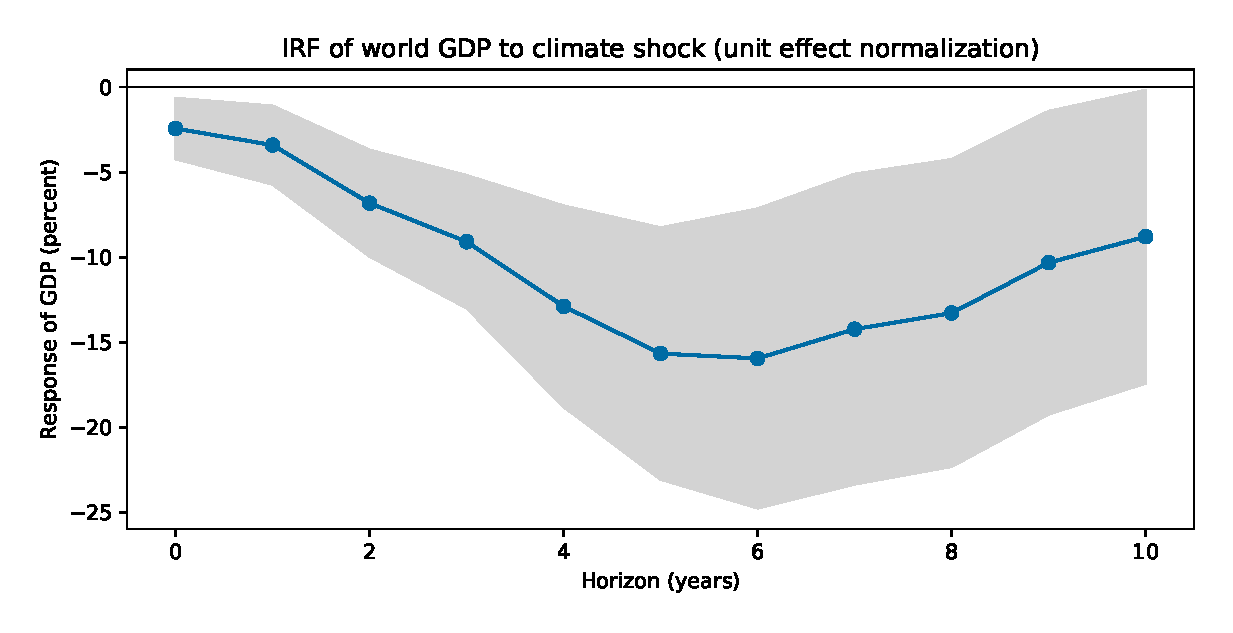
\includegraphics[width=\linewidth]{fig/bk_irf_unitnorm.eps}
\end{figure}
}

\frame{
\frametitle{Narrative restrictions}
\begin{itemize}
\item How to construct proxies in practice? One way is through qualitative \textbf{narrative restrictions}.
\item Suppose we have information about a subset of historical dates where there were especially large \emph{positive} or \emph{negative} shocks of a certain kind (e.g., monetary policy shocks). At other dates we're unsure.
\item Define (noisy) proxy:
\[z_t \equiv \begin{cases}
+1 & \text{if large, positive shock at time } t, \\
-1 & \text{if large, negative shock at time } t, \\
0 & \text{otherwise}.
\end{cases}\]
\vspace{-0.5\baselineskip}
\begin{itemize}
\item Relevance: $z_t$ is positively correlated with the shock of interest.
\item Dynamic exogeneity: $z_t$ is uncorrelated with the other economic shocks if (i) these other shocks do not influence which dates we have information on, and (ii) misclassifications are random.
\end{itemize}
\end{itemize}
}

\frame{
\frametitle{Weak instruments}
\begin{itemize}
\item If the normalization variable $\bar{y}_t$ is only weakly correlated with the proxy $z_t$ (conditional on controls), then we have a weak instrument.
\item There are two reasons why the IV could be weak:
\begin{enumerate}
\item The proxy $z_t$ is dominated by noise, so only weakly correlated with the shock of interest $\varepsilon_{1t}$.
\item The normalization variable $\bar{y}_t$ responds only weakly to the shock of interest $\varepsilon_{1t}$ on impact.
\end{enumerate}
\item We should pick a normalization variable that correlates strongly with the proxy.
\end{itemize}
}

\frame{
\frametitle{Small-sample bias of LP}
\begin{itemize}
\item Though the LP estimator is consistent under our assumptions, it can still be biased in small samples, similar to VAR estimators.
\item There exist various procedures for bias-correcting LP.
\item Bootstrap procedures can also improve the finite-sample coverage probability of the LP confidence interval.
\item For details, see the review article by Montiel Olea et al.\ (2026) on the reading list.
\end{itemize}
}

\frame{
\frametitle{Dynamic causal effects in panel data}
\begin{itemize}
\item Sometimes we have access to time series for many different economic \textbf{units}, like countries, sectors, firms, households, etc.
\item Let $y_{it}$ and $x_{it}$ be an outcome and a shock for unit $i$ at time $t$, where $i=1,\dots,n$ and $t=1,\dots,T$.
\item A \textbf{panel LP} estimates the impulse response of $y$ wrt.\ $x$ at horizon $h$ using a panel fixed effects regression
\[y_{i,t+h} = \hat{\nu}_i + \hat{\tau}_t + \hat{\beta}_h x_{it} + \hat{\bm{\delta}}_1'\bm{w}_{i,t-1} + \dots + \hat{\bm{\delta}}_p'\bm{w}_{i,t-p} + \hat{v}_{h,i,t+h}.\]
\vspace{-1.3\baselineskip}
\begin{itemize}
\item $\hat{\nu}_i$: unit fixed effects. These control for unobserved time-invariant heterogeneity across units.
\item $\hat{\tau}_t$: time fixed effects. These control for unobserved global factors that affect all units equally.
\item $\bm{w}_{it}$: vector of unit-specific control variables.
\end{itemize}
\end{itemize}
}

\frame{
\frametitle{Dynamic causal effects in panel data (cont.)}
\begin{itemize}
\item The regression on the previous slide assumes that the IRF is the same for all units.
\item Suppose instead we want to model the impulse responses as depending on an observed unit characteristic $s_i$.
\item We can model cross-unit heterogeneity in impulse responses using an interaction term:
{ \small
\[y_{i,t+h} = \hat{\nu}_i + \hat{\tau}_t + \alert{\hat{\beta}_h x_{it} + \hat{\varphi}_h (s_i-\bar{s}) x_{it}} + \hat{\bm{\delta}}_1'\bm{w}_{i,t-1} + \dots + \hat{\bm{\delta}}_p'\bm{w}_{i,t-p} + \hat{v}_{h,i,t+h},\]
}

where $\bar{s}\equiv \frac{1}{n}\sum_{i=1}^n s_i$.
\item Then the impulse response estimate for unit $i$ is
\[\tilde{\beta}_h(s_i) \equiv \hat{\beta}_h + \hat{\varphi}_h(s_i-\bar{s}).\]
\end{itemize}
}

\frame{
\frametitle{Panel data: hypothetical example}
{ \small
\[y_{i,t+h} = \hat{\nu}_i + \hat{\tau}_t + \alert{\hat{\beta}_h x_{it} + \hat{\varphi}_h (s_i-\bar{s}) x_{it}} + \hat{\bm{\delta}}_1'\bm{w}_{i,t-1} + \dots + \hat{\bm{\delta}}_p'\bm{w}_{i,t-p} + \hat{v}_{h,i,t+h}\]
}
\begin{itemize}
\item $y_{it}$: inflation rate of country $i$ at time $t$
\item $x_{it}$: monetary shock in country $i$ at time $t$
\item $\bm{w}_{it}$: real GDP, inflation, and monetary shock in country $i$ at time $t$
\item $s_i$: index of how independent the central bank in country $i$ is from the country's government
\item $\hat{\beta}_h$: estimated average impulse response (across countries)
\item $\hat{\varphi}_h$ measures whether monetary shocks have larger effect on inflation in countries with more independent central banks
\end{itemize}
}

\frame{
\frametitle{Panel data: aggregate shock}
\begin{itemize}
\item In some panel data applications, the shock $x_{it}$ is common to all units $i$, so $x_{it}=x_t$.
\item Example: panel data regressions in Bilal \& K\"{a}nzig (2026).
\begin{itemize}
\item $y_{it}$: log real GDP in country $i$ at time $t$.
\item $x_t$: \emph{global} temperature anomaly.
\end{itemize}
\item Since $x_t$ does not vary across units, it is perfectly multi-collinear with the time dummies. We therefore have to drop the latter if we want to identify the causal effects of $x_t$.
\item Panel regression with aggregate shock:
\[y_{i,t+h} = \hat{\nu}_i + \hat{\beta}_h x_t + \hat{\bm{\delta}}_1'\bm{w}_{i,t-1} + \dots + \hat{\bm{\delta}}_p'\bm{w}_{i,t-p} + \hat{v}_{h,i,t+h}.\]
\end{itemize}
}

\frame{
\frametitle{Panel data: aggregate shock (cont.)}
\[y_{i,t+h} = \hat{\nu}_i + \hat{\beta}_h x_t + \hat{\bm{\delta}}_1'\bm{w}_{i,t-1} + \dots + \hat{\bm{\delta}}_p'\bm{w}_{i,t-p} + \hat{v}_{h,i,t+h}\]
\begin{itemize}
\item $\bm{w}_{it}$ should include both unit-specific controls (e.g., $y_{it}$) and aggregate controls (e.g., $x_t$).
\begin{itemize}
\item Include the same aggregate controls you would use if it were a pure time series LP.
\end{itemize}
\item We could include an interaction term $(s_i-\bar{s}) \times x_t$ to estimate heterogeneous responses.
\item Standard errors should be clustered by time to allow for additional (unobserved) aggregate shocks. Need to control for sufficient lags $p$, as in pure time series LP.
\end{itemize}
}

\begin{frame}[fragile]
\codesize
\begin{verbatim}
# Load country panel data
df_panel = pd.read_csv('data/bilal_kaenzig2026_panel.csv')
df_panel = df_panel[df_panel['year'] >= 1960].copy()
df_panel = df_panel.set_index(['country_code', 'year']).sort_index()

# Avg temperature by country
df_panel['avgtemp'] = df_panel.groupby('country_code')['lctmp_bkly_pw'].transform('mean')

# Own lags of outcome (within country)
for l in range(1, nlag + 1):
    df_panel[f'lnrgdppc_pwt_lag{l}'] = (
        df_panel.groupby(level='country_code')['lnrgdppc_pwt'].shift(l)
    )

# Merge in aggregate shock + controls
df_panel = df_panel.join(df[['temp_anom'] + control_cols], on='year')
\end{verbatim}
\end{frame}

\begin{frame}[fragile]
\codesize
\begin{verbatim}
# Interaction term
avgtemp_global = df_panel.groupby(level='country_code')['avgtemp'].first().mean()
df_panel['avgtemp_d'] = df_panel['avgtemp'] - avgtemp_global # de-mean
df_panel['temp_anom_x_avgtemp'] = df_panel['temp_anom'] * df_panel['avgtemp_d']

# Panel LP with unit FE and time-clustered SE
own_lag_cols = [f'lnrgdppc_pwt_lag{l}' for l in range(1, nlag + 1)]
panel_regs = own_lag_cols + ['temp_anom', 'temp_anom_x_avgtemp'] + control_cols

irf_panel = np.empty(max_horizon + 1)
se_panel  = np.empty(max_horizon + 1)
inter_panel = np.empty(max_horizon + 1)
inter_se_panel = np.empty(max_horizon + 1)
for h in range(max_horizon + 1):
    y = df_panel.groupby(level='country_code')['lnrgdppc_pwt'].shift(-h)
    reg = PanelOLS(y, df_panel[panel_regs], entity_effects=True
                   ).fit(cov_type='clustered', cluster_time=True)
    irf_panel[h] = reg.params['temp_anom']
    se_panel[h]  = reg.std_errors['temp_anom']
    inter_panel[h] = reg.params['temp_anom_x_avgtemp']
    inter_se_panel[h] = reg.std_errors['temp_anom_x_avgtemp']
\end{verbatim}
\end{frame}

\frame{
\begin{figure}
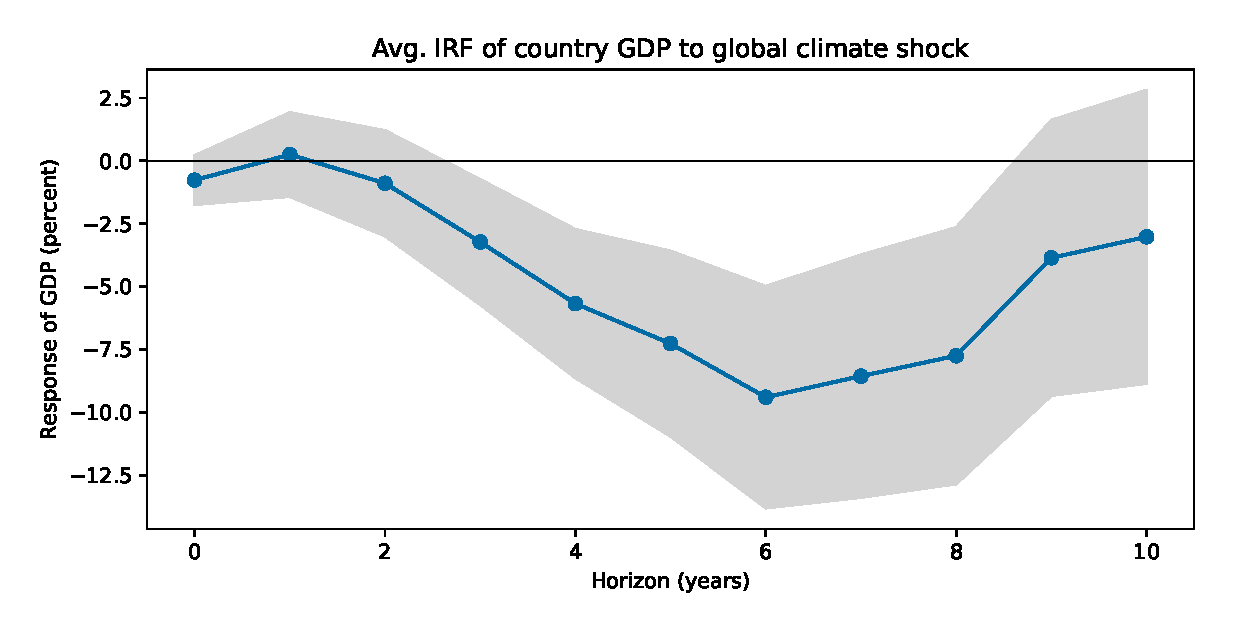
\includegraphics[width=\linewidth]{fig/bk_irf_panel.eps}
\end{figure}
}

\begin{frame}[fragile]
\begin{verbatim}
     beta  beta_se    phi  phi_se
h                                
0  -0.768    0.979 -0.243   0.160
1   0.247    1.677 -0.406   0.257
2  -0.892    2.106 -0.538   0.327
3  -3.228    2.498 -0.570   0.349
4  -5.678    2.965 -0.624   0.389
5  -7.268    3.702 -0.720   0.417
6  -9.399    4.429 -0.801   0.412
7  -8.561    4.848 -0.722   0.423
8  -7.750    5.124 -0.749   0.411
9  -3.858    5.503 -0.822   0.359
10 -3.023    5.861 -0.799   0.348
\end{verbatim}
\medskip
{\tt beta}: avg.\ impulse response \\
{\tt phi}: coef.\ on interaction $(s_i-\bar{s})\times x_t$
\end{frame}

\frame{
\frametitle{What did we learn?}
\begin{itemize}
\item FEVD
\item Identification from proxy variables
\begin{itemize}
\item Measurement error
\item LP-IV
\item Narrative proxies
\end{itemize}
\item LP small-sample bias
\item Panel LP
\begin{itemize}
\item Idiosyncratic vs.\ aggregate shocks
\item Interaction terms
\end{itemize}
\end{itemize}
}

\frame{
\frametitle{Looking ahead}
\begin{itemize}
\item If we believe the data is well described by a VAR model, can we use that to improve our estimates of IRFs and FEVDs?
\item How do LP and VAR estimates compare?
\item Yet more ways of identifying unobserved shocks
\end{itemize}
}

\end{document}
